\begin{enumerate}
	\item L'utilisateur clique sur son nom dans la bar de navigation.
	\item L'utilisateur est redirigé vers sa page de profil. 
	\item L'utilisateur retrouve l'information dans le cadre afficher sur la page.
\end{enumerate}

\vspace{\baselineskip}
\begin{figure}[h]
	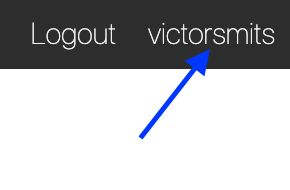
\includegraphics[width=0.5\textwidth,center]{Figures/us7-1}
	\caption{Bouton de navigation vers le profil}
\end{figure}

\vspace{\baselineskip}
\begin{figure}[h]
	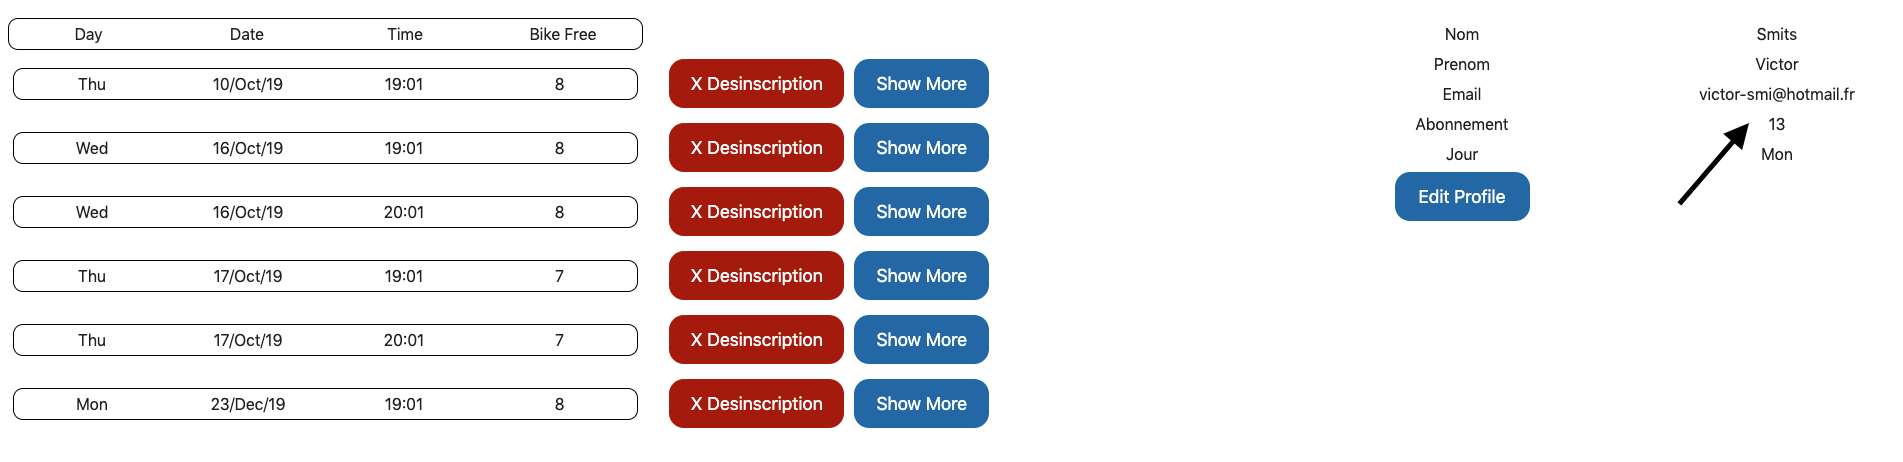
\includegraphics[width=0.9\textwidth,center]{Figures/us7-2}
	\caption{Nombre de séance restante dans l'abonnement}
\end{figure}


\vspace{\baselineskip}
\subsubsection{Script concernés}
	\begin{itemize}
		\item \href{https://github.com/victorsmits/Aquabike/blob/master/backend/src/Controller/ProfileController.php}{ProfileController.php}
		\item \href{https://github.com/victorsmits/Aquabike/blob/master/backend/templates/registration/profile.html.twig}{profile.html.twig}
		\item \href{https://github.com/victorsmits/Aquabike/blob/master/backend/src/Entity/Person.php}{Person.php}
	\end{itemize}
